%% main_v18.tex — NeurIPS 2026 submission, v1.8
%% Compile: pdflatex main_v18 && bibtex main_v18 && pdflatex main_v18 && pdflatex main_v18

\documentclass{article}

\PassOptionsToPackage{numbers,sort&compress}{natbib}
\usepackage[final,main]{neurips_2026}

\usepackage{amsmath,amssymb,amsthm,mathtools}
\usepackage{booktabs,multirow,array,tabularx}
\usepackage{graphicx,subcaption}
\usepackage{adjustbox}
\usepackage{placeins}
\graphicspath{{./}{../figures/}}
\usepackage{xcolor}
\usepackage[colorlinks=true,linkcolor=blue!70!black,citecolor=blue!70!black,
            urlcolor=blue!70!black]{hyperref}
\usepackage{algorithm,algpseudocode}
\usepackage[utf8]{inputenc}
\usepackage[T1]{fontenc}
\usepackage{microtype,enumitem,xspace,nicefrac}

\newcommand{\reff}{\ensuremath{r_{\mathrm{eff}}}\xspace}
\newcommand{\SAk}{\ensuremath{\mathrm{SA}_k}\xspace}
\newcommand{\UID}{\ensuremath{\mathrm{UID}}\xspace}
\newcommand{\SSRdag}{\ensuremath{\mathrm{SSR}^{\ddagger}}\xspace}
\newcommand{\rhoSp}{\ensuremath{\rho_{\mathrm{Sp}}}\xspace}

\newtheorem{theorem}{Theorem}
\newtheorem{lemma}{Lemma}
\newtheorem{proposition}[lemma]{Proposition}
\newtheorem{observation}[lemma]{Observation}
\newtheorem{corollary}[lemma]{Corollary}
\newtheorem{remark}{Remark}
\newtheorem{definition}{Definition}

\title{Width Confounding in Label-Free Cross-Architecture Model Selection:\\
       Diagnosis and Subspace Correction}

\author{%
  Qin Liu \quad Chen Zhong \quad Fengshan Zhao\thanks{Corresponding author: Fengshan Zhao, \texttt{fs.zhao@nju.edu.cn}}\\
  State Key Laboratory of Novel Software Technology\\
  Nanjing University, Nanjing, China
}
\hypersetup{unicode=true,
  pdftitle={Width Confounding in Label-Free Cross-Architecture Model Selection: Diagnosis and Subspace Correction},
  pdfauthor={Qin Liu, Chen Zhong, Fengshan Zhao}}
\date{}

\begin{document}
\maketitle

\begin{abstract}
Choosing a pretrained encoder without target labels is a practical problem in transfer learning. RankMe, validated primarily within architecture families, can be confounded by feature width when architectures differ. Under an isotropic random-feature model at fixed aspect ratio, its effective rank scales as $\Theta(d)$. We propose Subspace-Corrected Ranking (SCR), which augments the target spectrum with the alignment between target and reference features extracted by the same candidate encoder. Its default member \SSRdag\ subtracts log subspace alignment from log effective rank. Across $22$ pool--task units from three heterogeneous model pools (MV/VTAB/EX), \SSRdag\ reduces mean selection regret from $0.133$ to $0.069$ relative to RankMe (paired difference: $-0.0645$; target-name-clustered $95\%$ CI: $[-0.122,-0.020]$). On MV, the mean score--width correlation decreases from $0.609$ to $0.305$, indicating that width dependence is reduced but remains present. On five MV tasks, a two-stage pipeline using \SSRdag\ for architecture selection and RankMe for within-family selection requires fewer candidate evaluations while achieving regret similar to evaluating \SSRdag\ over all candidates.
\end{abstract}

\section{Introduction}
\label{sec:intro}

Transfer learning starts with a choice: which pretrained encoder to transfer to the target task. When candidate encoders share the same architecture but differ in pretraining recipe, the choice can be made cheaply via a label-free score on the encoder's penultimate features. The dominant such score, \emph{RankMe} \citep{garrido2023rankme}, computes the effective rank $\reff(H)$ of the feature matrix and ranks candidates by $\log\reff$. In the within-architecture setting where RankMe was validated, the penultimate-layer dimension $d$ is constant across candidates, so width alone cannot explain their ranking.

A practitioner using timm \citep{wightman2019timm} or torchvision compares heterogeneous backbones, including ResNet \citep{he2016resnet}, ViT \citep{dosovitskiy2021vit}, ConvNeXt \citep{liu2022convnext}, and EfficientNet \citep{tan2019efficientnet}, whose feature widths vary substantially. The within-family setting in which RankMe was validated does not establish its reliability across these architectures. On the $119$-candidate multi-variant (MV) pool (Section~\ref{sec:setup}), RankMe is width-associated (mean per-task $\rhoSp=0.609$), with regret $0.144$: better than random ($0.191$), but worse than our relational score \SSRdag\ ($0.098$; Section~\ref{sec:ssr}). On the Visual Task Adaptation Benchmark (VTAB) and extended (EX) pools, however, RankMe has higher mean regret than random. Taken together, these results show that width association alone does not determine whether selection is better or worse than random.

The mechanism is a consequence of RankMe's target-only spectral form under feature isotropy. A Marchenko--Pastur argument shows that RankMe effective rank scales as $\Theta(d)$ at fixed positive aspect ratio, so $\log\reff$ equals $\log d$ plus an aspect-ratio-dependent constant asymptotically. This formal statement is specific to RankMe; rotation invariance alone is insufficient to conclude that an arbitrary score is monotone in $d$.

Figure~\ref{fig:method_overview} summarizes our approach. Given unlabeled target images and a fixed, target-disjoint reference dataset, each candidate encoder separately maps both datasets into its own feature space. SCR augments the target spectrum with the relative geometry of these two subspaces; its default member \SSRdag\ subtracts log alignment from log effective rank. Only the resulting scalar scores are compared across encoders, so their feature dimensions need not match. This provides a label-free way to shortlist pretrained backbones before labeled downstream evaluation. Across $22$ common-support pool--task units from MV, VTAB, and EX, \SSRdag\ reduces mean selection regret from $0.133$ for RankMe to $0.069$, showing that target--reference subspace geometry can improve upon target-spectrum-only selection on these pools.

\begin{figure}[t]
\centering
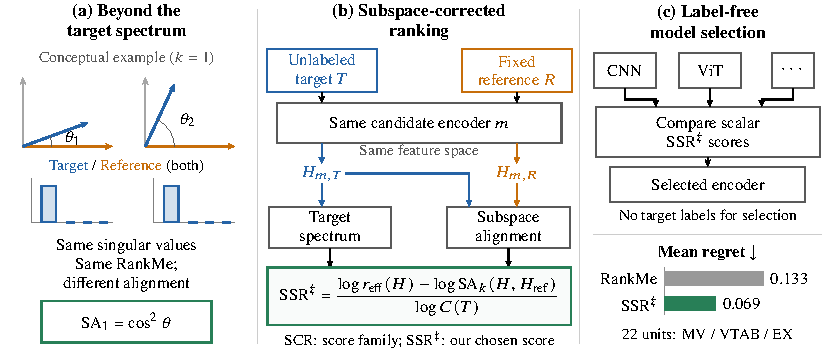
\includegraphics[width=\linewidth]{fig_method_overview.pdf}
\caption{Overview of subspace correction. (a) Equal target spectra can have different reference-relative angles; this is not an accuracy ordering. (b) Alignment uses both feature matrices from the same candidate, with $H=H_{m,T}$ and $H_{\mathrm{ref}}=H_{m,R}$. Class-count metadata $C(T)>1$ only rescales within-task scores; omitting it leaves ranking unchanged. (c) Scalar scores enable zero-target-label selection. Bars summarize $22$ common-support units (Table~\ref{tab:crosspool}); target labels are used only for evaluation.}
\label{fig:method_overview}
\end{figure}

\paragraph{Contributions.}
\textbf{(i) Diagnosis.} We identify feature-width confounding in RankMe across heterogeneous architectures and explain its effective-rank scaling under an isotropic random-feature model.
\textbf{(ii) Subspace correction.} We introduce Subspace-Corrected Ranking (SCR), a family of label-free relational scores that complements the target spectrum with within-encoder target--reference geometry. Its default member, \SSRdag, reduces mean selection regret relative to RankMe on the evaluated common support.
\textbf{(iii) Budgeted selection.} We evaluate a two-stage pipeline that uses \SSRdag\ for architecture selection and RankMe for within-family variant selection, which on five MV tasks uses fewer candidate evaluations at regret similar to flat \SSRdag.

\section{Related Work}
\label{sec:related}

\textbf{Transferability scores.} RankMe \citep{garrido2023rankme} ranks pretrained encoders by the effective rank of penultimate features, using $p_i=\sigma_i/\sum_j\sigma_j$; our focus is the heterogeneous-pool setting beyond its original within-family validation. VNE \citep{kim2023vne} uses the entropy of normalized squared singular values, but we do not extend our RankMe-specific theorem to VNE. Official classification DiSCO \citep{zhang2025disco} uses target ground-truth labels to construct class-conditional quantities and is therefore reported as a label-dependent comparator, not a zero-label baseline. Other label-requiring scores include LogME \citep{zhang2021logme}, H-score \citep{bao2019hscore}, NCTI \citep{wang2023ncti}, LEEP \citep{nguyen2020leep}, N-LEEP \citep{li2021nleep}, PACTran \citep{ding2022pactran}, OTCE \citep{tan2021otce}, GBC \citep{pandy2022gbc}, TransRate \citep{huang2022transrate}, NCE \citep{tran2019nce}, and Task2Vec \citep{achille2019task2vec}. Transfer learning more broadly is surveyed in \citet{pan2010transfer}.

\textbf{Subspace alignment and random matrix theory.}  Subspace alignment \citep{fernando2013sa} was introduced for unsupervised domain adaptation via principal-angle geometry on the Grassmann manifold \citep{hamm2008grassmann}.  Neural network representation similarity via CKA and SVCCA \citep{kornblith2019similarity,raghu2017svcca} uses related geometric ideas to compare layers; we use principal-angle geometry differently, as a label-free measure of generic-vs-specific feature structure relative to a fixed reference dataset encoded by each candidate.  The Marchenko--Pastur law \citep{marchenko1967distribution} has been applied to characterize weight matrices in deep networks \citep{martin2021implicit}; we apply it directly to feature matrices to derive the width-confound mechanism.

\textbf{Two-stage and budgeted model selection.}  Staged screening followed by precise evaluation is a standard design in neural architecture search and Bayesian hyperparameter optimization.  In source-free transferability estimation \citep{zhang2021logme,wang2023ncti}, the same logic supports a cross-architecture stage at low cost followed by a within-family stage; we evaluate this design and a mixed-budget extension as five-task proofs of concept.

\section{Setup}
\label{sec:setup}

\textbf{Pools.} Table~\ref{tab:pool_setup} summarizes the four pools (Appendices~B--E). MV uses timm/torchvision \citep{wightman2019timm}; its $119$ variants in $35$ multi-variant groups form the headline and two-stage support. VTAB \citep{zhai2019large} has $24$ complete architectures; excluding the STL-10 reference leaves seven targets. SSL has eight encoders, including CLIP \citep{radford2021clip}, DINOv2 \citep{oquab2023dinov2}, DINO \citep{caron2021dino}, and MoCo \citep{he2020moco}, on $29$ tasks with incomplete support. EX has $51$ supervised timm variants from $35$ architectures on ten tasks. The inventories cover $52$ task units and $d\in[192,4096]$.

\begin{table}[h]
\centering\small
\caption{Four architecturally distinct evaluation pools used throughout the paper.  Width ranges describe the candidate pools; they are not a validated score-selection threshold.}
\label{tab:pool_setup}
\begin{adjustbox}{max width=\linewidth}
\begin{tabular}{lccccc}
\toprule
Pool & Archs & Variants & Tasks & $d$ range & $d_{\max}/d_{\min}$ \\
\midrule
MV pool (multi-variant)  & $35$ / $48$ full & $119$ (multi-var.) / $132$ (full) & $5$  & $[192, 4096]$ & $21.3\times$ \\
VTAB pool                & $24$ & $24$                               & $8$  & $[192, 2048]$ & $10.7\times$ \\
SSL/multimodal pool      & $8$  & $8$                                & $29$ & $[384, 2048]$ & $5.3\times$  \\
EX pool (supv.)          & $35$ & $51$                               & $10$ & $[192, 4096]$ & $21.3\times$ \\
\bottomrule
\end{tabular}
\end{adjustbox}
\end{table}

\textbf{Scores.} Effective rank $\reff$ follows RankMe \citep{garrido2023rankme}: $p_i=\sigma_i/\sum_j\sigma_j$ and $\reff=\exp(-\sum_i p_i\log p_i)$. For each candidate encoder $m$ in the main $22$-unit comparison, $\SAk$ compares its target features with its STL-10 features; both are produced by encoder $m$ and therefore share dimension $d_m$. We use uncentered feature matrices, default $k=20$, and clip quantities to at least $10^{-12}$ before taking logarithms. Different candidates' subspaces are never compared directly. Official classification DiSCO and the other label-requiring methods are reported separately from the zero-label RankMe--\SSRdag\ comparison.

\textbf{Linear-probe ground truth.} We use held-out accuracy of $\ell_2$-regularized logistic regression ($C=1$) on an $80/20$ split. Regret is the gap to the oracle over the same candidate set. The $22$-unit paired and target-name-clustered bootstrap and the five-task pipeline intervals each use $100{,}000$ resamples with seed $42$.

\textbf{Feature extraction and preprocessing.} For torchvision VGG16/VGG16-BN, we retain the hidden fully connected layers to obtain $4096$-dimensional features and apply the official weights transform once to target and STL-10 images. The other $23$ torchvision variants in the $119$-candidate support retain cached features associated with an extractor that applies loader resizing, cropping, and normalization before the weights transform, including a second normalization. These include the SVHN oracle, DenseNet-169. Individual historical cache provenance is incomplete. A VGG control retaining this two-transform pipeline gives identical $22$-unit RankMe/\SSRdag\ regrets, but does not validate preprocessing for the remaining candidates. The benchmark is not a uniformly preprocessed comparison; its oracles and uncertainty are conditional on the retained features (Appendices~B and~G).

\section{The Width Confound}
\label{sec:theory}

We isolate the failure mechanism with two formal statements. Both proofs are in Appendix~A.

\begin{lemma}[Marchenko--Pastur scaling]
\label{lem:mp}
Let $H \in \mathbb{R}^{n\times d}$ have i.i.d.\ rows from $\mathcal{N}(0,\sigma^2 I_d)$, with $\sigma>0$. As $n,d\to\infty$ with $\gamma = n/d\in(0,\infty)$ fixed,
$\reff(H)/d \to c(\gamma) > 0$ almost surely, where $c(\gamma)$ depends only on the aspect ratio.  In particular $\reff(H) = \Theta(d)$.
\end{lemma}

\textbf{Why width enters.} Let $\lambda_i=\sigma_i^2/(n\sigma^2)$ include all $d$ eigenvalues, and set $S_d=d^{-1}\sum_i\sqrt{\lambda_i}$. RankMe's singular-value normalization gives the exact identity
\[
 \log\reff(H)=\log d+\log S_d
 -\frac{1}{2S_d d}\sum_i\sqrt{\lambda_i}\log\lambda_i.
\]
At fixed aspect ratio, the last two terms converge to a finite constant under the stated Gaussian model. The continuous extension $\sqrt{x}\log x\to0$ as $x\downarrow0$ handles zero eigenvalues; no spectral gap from zero is assumed. Thus width contributes the explicit $\log d$ term. This is an explanatory model, not an assertion that every pretrained representation is isotropic; equal classwise total variances do not establish directional isotropy. Appendix~A gives the full derivation.

\begin{proposition}[\SSRdag\ is relational and jointly basis-invariant]
\label{prop:nonrot}
For candidate encoder $m$, take the retained right-singular subspaces to be uniquely specified (or transport a chosen subspace consistently through a tied singular-value block). For $Q\in O(d_m)$, jointly replacing $(H_{m,T},H_{m,R})$ by $(H_{m,T}Q,H_{m,R}Q)$ leaves their principal angles, $\SAk$, and \SSRdag\ unchanged. In general, \SSRdag\ is not determined by the singular values of $H_{m,T}$ alone: it additionally depends on the relative geometry of the target and reference right-singular subspaces.
\end{proposition}

\textbf{Why the correction adds information.} Under the common basis change, $V_T'=Q^\top V_T$ and $V_R'=Q^\top V_R$, so $(V_T')^\top V_R'=V_T^\top V_R$. By contrast, Figure~\ref{fig:method_overview}(a) holds a rank-one reference fixed while rotating a rank-one target without changing its singular value. With one retained direction ($k=1$), alignment is $\cos^2\theta$: RankMe cannot distinguish the two targets, whereas \SSRdag\ can. This illustrates information beyond the target spectrum, not an ordering of their downstream accuracies.



\textbf{Finite-pool illustration.} Figure~\ref{fig:reff_d} uses RankMe's singular-value normalization consistently with the headline scores. After averaging within architecture groups, effective rank and width have Spearman correlations $+0.877$ on VTAB and $+0.871$ on EX. These finite-pool associations are distinct from per-task correlations and do not constitute a fitted asymptotic law.

\begin{figure}[t]
\centering
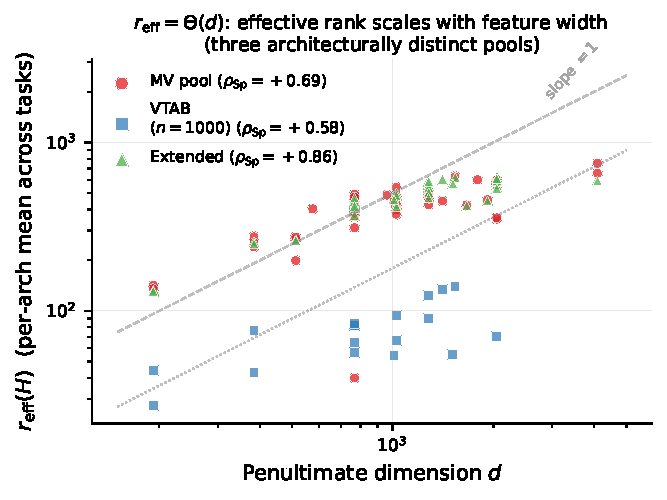
\includegraphics[width=0.64\linewidth]{fig_reff_d_scatter.pdf}
\caption{Effective rank versus feature width for the $24$ VTAB and $35$ EX architecture groups. The dashed slope-$1$ line is a visual guide, not a fit. VTAB includes its eight cached datasets for this spectral diagnostic only; STL-10 is excluded from all target-selection comparisons.}
\label{fig:reff_d}
\end{figure}

\textbf{Empirical association across pools.} Mean per-task $\rhoSp(\mathrm{RankMe},d)$ is $0.609$ on MV, $0.879$ on VTAB, and $0.766$ on EX; width--LP correlations are $-0.049$, $+0.233$, and $-0.070$. Thus width association is not equivalent to quality prediction. MV RankMe is better than random, whereas VTAB and EX have higher mean regret than their respective random baselines (Table~\ref{tab:pool_diagnosis}). On the same $119$-candidate MV support, \SSRdag\ reduces mean score--width correlation to $0.305$ (task range $0.156$--$0.495$) and increases mean score--LP correlation from $0.352$ to $0.512$. This is descriptive evidence of reduced, not eliminated, width dependence; it does not isolate a causal effect of width. On EX, mean Kendall correlation between RankMe and $d$ is $\tau=+0.618$ across $10$ tasks.

\begin{table}[htbp]
\centering\small
\caption{Width and quality diagnostics by pool. MV uses 119 candidates; VTAB excludes STL-10. Correlations are per-task Spearman means.}
\label{tab:pool_diagnosis}
\setlength{\tabcolsep}{4pt}
\resizebox{\linewidth}{!}{%
\begin{tabular}{lrrrrr}
\toprule
Pool & Groups/tasks & $\rho(\mathrm{RankMe},d)$ & $\rho(d,\mathrm{LP})$ & RM regret & Random regret \\
\midrule
MV & $35/5$ & $0.609$ & $-0.049$ & $0.144$ & $0.191$ \\
VTAB & $24/7$ & $0.879$ & $0.233$ & $0.110$ & $0.106$ \\
EX & $35/10$ & $0.766$ & $-0.070$ & $0.144$ & $0.131$ \\
\bottomrule
\end{tabular}}
\end{table}


\textbf{VTAB per-task breakdown.}  Table~\ref{tab:vtab_pertask} uses the same $24$ candidates for every non-reference target. The RankMe--width correlation ranges from $0.838$ to $0.915$, while regret varies substantially by task.

\begin{table}[h]
\centering\small
\caption{VTAB per-task width confound on the complete $24$-architecture support. STL-10 is excluded because it is the reference dataset.}
\label{tab:vtab_pertask}
\begin{tabular}{lrrl}
\toprule
Task & $\rhoSp(\mathrm{RankMe}, d)$ & Regret & RankMe pick \\
\midrule
CIFAR-10       & $+0.865$ & $+0.050$ & efficientnet\_b3 ($d{=}1536$) \\
CIFAR-100      & $+0.869$ & $+0.235$ & efficientnet\_b3 ($d{=}1536$) \\
DTD            & $+0.877$ & $+0.095$ & resnet101 ($d{=}2048$) \\
Fashion-MNIST  & $+0.886$ & $+0.045$ & wide\_resnet50\_2 ($d{=}2048$) \\
Flowers-102    & $+0.838$ & $+0.165$ & efficientnet\_b3 ($d{=}1536$) \\
Pets           & $+0.902$ & $+0.070$ & mobilenetv3\_large ($d{=}1280$) \\
SVHN           & $+0.915$ & $+0.110$ & efficientnet\_b3 ($d{=}1536$) \\
\midrule
\textbf{Mean}  & $\mathbf{+0.879}$ & $\mathbf{+0.110}$ & --- \\
\bottomrule
\end{tabular}
\end{table}

\textbf{VGG sensitivity and task variation.} Removing the three VGG variants ($3/119\approx2.5\%$) leaves RankMe and \SSRdag\ regrets unchanged at $0.144$ and $0.098$. RankMe selects a ResNeXt variant on four tasks and Inception on SVHN. \SSRdag\ improves over RankMe on four tasks, but is worse on SVHN; it is within $0.07$ LP of the oracle on two tasks (Table~\ref{tab:main_pertask}).

\begin{table}[htbp]
\centering\small
\caption{Per-task LP on 119 MV candidates. Random is the exact expectation. \SSRdag improves over RankMe on four tasks, but is worse on SVHN. EuroSAT also has a tied ViT-large oracle (LP 0.955).}
\label{tab:main_pertask}
\setlength{\tabcolsep}{4pt}
\resizebox{\linewidth}{!}{%
\begin{tabular}{lrrrrrrr}
\toprule
Task & Oracle & Random & RM & \SSRdag & RM group & \SSRdag group & Oracle group \\
\midrule
CIFAR-10 & $0.970$ & $0.787$ & $0.845$ & $0.870$ & resnext50 & resnet50 & convnext\_base \\
CIFAR-100 & $0.825$ & $0.486$ & $0.535$ & $0.670$ & resnext50 & resnet152 & convnext\_base \\
DTD & $0.740$ & $0.564$ & $0.625$ & $0.720$ & resnext50 & convnext\_base & convnext\_base \\
EuroSAT & $0.955$ & $0.882$ & $0.880$ & $0.905$ & resnext50 & efficientnet\_b3 & densenet201 (tie) \\
SVHN & $0.615$ & $0.428$ & $0.500$ & $0.450$ & inception\_v3 & efficientnet\_b3 & densenet169 \\
\bottomrule
\end{tabular}}
\end{table}


\textbf{Spectral truncation diagnostic.} One CIFAR-10 cell lacks truncated and auxiliary scores. For these comparisons only, we remove that variant uniformly, giving $118$ candidates on all five tasks. On this complete support, truncation at $D=128/256/512/768$ gives regrets $0.134/0.134/0.151/0.142$, versus full-spectrum RankMe $0.144$ and \SSRdag\ $0.098$. Some cutoffs improve RankMe, but all four have higher regret than \SSRdag. The cutoff is an additional design choice (Appendix~E).

\textbf{Auxiliary comparisons.} Table~\ref{tab:sota_flat} reports regret and Table~\ref{tab:vgg_sensitivity} mean LP on $118$ candidates, or $115$ without VGG. Removing VGG lowers LogME accuracy, while H-score is unchanged. Direct dimension normalization, $\log\reff-\log d$, gives regret $0.200$, versus random $0.192$ and \SSRdag\ $0.098$ on the same $118$ candidates; subtracting $\log d$ is insufficient here. The LEEP column is a clustering proxy, not an official LEEP implementation. These diagnostics do not extend our RankMe-specific theorem.

\begin{table}[htbp]
\centering\small
\caption{Complete auxiliary support: 118 candidates after excluding one variant with a missing score; 115 after also removing three VGG variants. Entries are five-task mean regret.}
\label{tab:sota_flat}
\setlength{\tabcolsep}{4pt}
\resizebox{\linewidth}{!}{%
\begin{tabular}{lrrrr}
\toprule
Method & With VGG & Without VGG & $\Delta$ & Type \\
\midrule
Random & $0.192$ & $0.191$ & $-0.001$ & reference \\
RankMe & $0.144$ & $0.144$ & $0.000$ & zero-label \\
RankMe $(-\log d)$ & $0.200$ & $0.200$ & $0.000$ & zero-label \\
LogME & $0.219$ & $0.550$ & $0.331$ & labels \\
H-score & $0.470$ & $0.470$ & $0.000$ & labels \\
NCTI & $0.155$ & $0.155$ & $0.000$ & labels \\
\SSRdag & $0.098$ & $0.098$ & $0.000$ & zero-label \\
LEEP clustering proxy & $0.038$ & $0.038$ & $0.000$ & labels \\
\bottomrule
\end{tabular}}
\end{table}


\begin{table}[htbp]
\centering\small
\caption{Complete auxiliary support: 118 candidates after excluding one variant with a missing score; 115 after also removing three VGG variants. Entries are five-task mean LP.}
\label{tab:vgg_sensitivity}
\setlength{\tabcolsep}{4pt}
\resizebox{\linewidth}{!}{%
\begin{tabular}{lrrrr}
\toprule
Method & With VGG & Without VGG & $\Delta$ & Type \\
\midrule
Random & $0.629$ & $0.630$ & $0.001$ & reference \\
RankMe & $0.677$ & $0.677$ & $0.000$ & zero-label \\
RankMe $(-\log d)$ & $0.621$ & $0.621$ & $0.000$ & zero-label \\
LogME & $0.602$ & $0.271$ & $-0.331$ & labels \\
H-score & $0.351$ & $0.351$ & $0.000$ & labels \\
NCTI & $0.666$ & $0.666$ & $0.000$ & labels \\
\SSRdag & $0.723$ & $0.723$ & $0.000$ & zero-label \\
LEEP clustering proxy & $0.783$ & $0.783$ & $0.000$ & labels \\
\bottomrule
\end{tabular}}
\end{table}


\section{Subspace-Corrected Ranking}
\label{sec:ssr}

\textbf{Geometric premise.} For candidate encoder $m$, write $H=H_{m,T}$ and $H_{\mathrm{ref}}=H_{m,R}$ for its target and fixed-reference feature matrices. Let $V_{m,\mathrm{ref},1:k}$ contain the top-$k$ right singular vectors of $H_{\mathrm{ref}}$, and write $P = V_{m,\mathrm{ref},1:k} V_{m,\mathrm{ref},1:k}^\top$, $Q = I - P$. Let $\Sigma_B$ be the class-frequency-weighted covariance of target class means, computed with target labels only for this diagnostic. Define
\[
  f_{\mathrm{spe}}(H, H_{\mathrm{ref}}) := \frac{\mathrm{tr}(Q\Sigma_B Q)}{\mathrm{tr}(\Sigma_B)},
\]
the fraction of between-class covariance lying outside the same candidate's reference-data subspace. This residual fraction does not, by itself, establish architecture-specific information or compare different encoders. On the complete VTAB support ($24{\times}7=168$ architecture--task pairs), the subspace alignment $\SAk(H, H_{\mathrm{ref}})$ is nearly perfectly anti-correlated with $f_{\mathrm{spe}}$ ($\rhoSp = -0.959$, Figure~\ref{fig:sigma_b_flow}). Within each task, $f_{\mathrm{spe}}$ is positively associated with LP accuracy (mean Spearman $\rho = +0.420$). Subtracting subspace alignment is therefore an empirically motivated, label-free penalty for overlap with the reference-data subspace; this observation is mechanistic evidence rather than a downstream guarantee. We exclude \texttt{resnet152} uniformly because reference and target features are available for only one of the eight VTAB datasets; all $168$ pairs on the resulting $24$-architecture support are computed successfully (see \texttt{results/camera\_ready/vtab\_fspe\_24arch\_uncentered.csv}).

\begin{figure}[t]
\centering
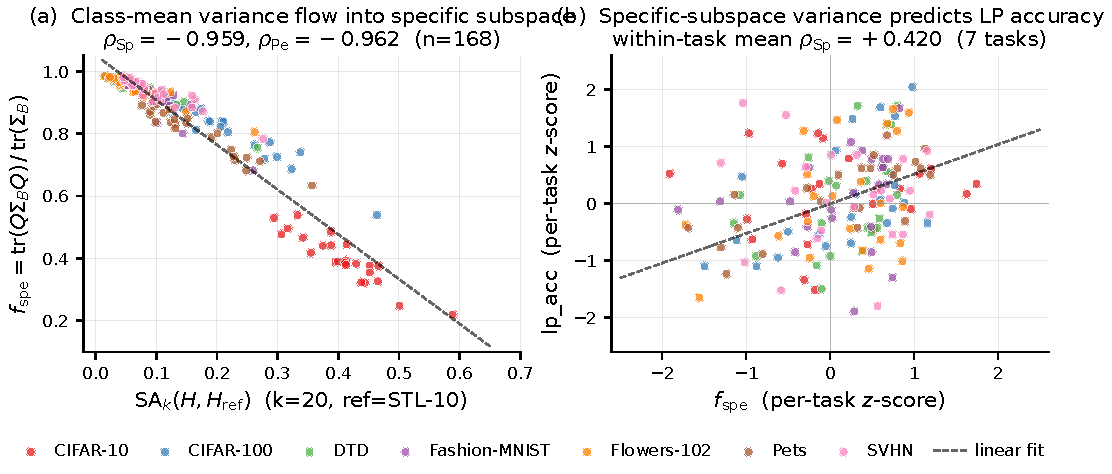
\includegraphics[width=0.92\linewidth]{fig_sigma_b_flow.pdf}
\caption{(a) Alignment between target and STL-10 features from the same candidate is nearly perfectly anti-correlated with the fraction of class-mean variance outside that candidate's reference-data subspace, $f_{\mathrm{spe}}$. (b) Within-task, $f_{\mathrm{spe}}$ is positively associated with linear-probe accuracy (mean Spearman $\rho=+0.420$ over seven tasks).}
\label{fig:sigma_b_flow}
\end{figure}

\textbf{Alignment and algorithm.} For candidate $m$, let the uncentered feature matrices be $H_{m,T}\in\mathbb{R}^{n_T\times d_m}$ and $H_{m,R}\in\mathbb{R}^{n_R\times d_m}$, both produced by encoder $m$. Let $V_T,V_R\in\mathbb{R}^{d_m\times k_m}$ contain their leading right-singular vectors, where $k_m=\min\{k,n_T,n_R,d_m\}$ and $k=20$ by default. With principal angles $\theta_1,\ldots,\theta_{k_m}$,
\[
 \SAk(H_{m,T},H_{m,R})
 =\frac{1}{k_m}\lVert V_T^\top V_R\rVert_F^2
 =\frac{1}{k_m}\sum_{i=1}^{k_m}\cos^2\theta_i.
\]
Algorithm~\ref{alg:ssr_score} gives the complete computation. Candidate feature dimensions may differ, because no cross-candidate subspaces are compared.

\begin{algorithm}[t]
\caption{Zero-label \SSRdag\ scoring for one candidate}
\label{alg:ssr_score}
\begin{algorithmic}[1]
\Require Encoder $m$; nonempty unlabeled target $T$ and target-disjoint reference $R$ with nonzero features; $k=20$; $\epsilon=10^{-12}$
\State Extract $H_{m,T}$ and $H_{m,R}$ with the same encoder and its fixed preprocessing; cache reference features.
\State Compute uncentered thin SVDs of both matrices, retaining target singular values $\{\sigma_i\}$.
\State Set $k_m=\min\{k,n_T,n_R,d_m\}$ and retain right-singular bases $V_T,V_R$ with $k_m$ columns.
\State $s\gets \lVert V_T^\top V_R\rVert_F^2/k_m$.
\State $p_i\gets \sigma_i/\sum_j\sigma_j$; $r\gets\exp(-\sum_{i:p_i>0}p_i\log p_i)$.
\State $a\gets\log\max(r,\epsilon)-\log\max(s,\epsilon)$.
\State \Return $a/\log C(T)$ if class-count metadata $C(T)>1$ is provided; otherwise return $a$ for identical per-task ranking.
\end{algorithmic}
\end{algorithm}

\textbf{Method family.} Subspace-Corrected Ranking is the family
\[
  \mathrm{SCR}(H, T; \beta, g) :=
  \frac{\log\reff(H) + \beta\cdot g\bigl(\SAk(H, H_{\mathrm{ref}})\bigr)}
       {\log C(T)},
\]
where $g$ is a monotonically decreasing function and $\beta \geq 0$.  Choosing $g(s) = -\log s$ with $\beta = 1$ gives
\[
  \SSRdag(H, T) := \frac{\log\reff(H) - \log\SAk(H, H_{\mathrm{ref}})}{\log C(T)},
\]
and $g(s)=1-s$ gives an additive variant. For per-task ranking, the common positive factor $1/\log C(T)$ may be omitted without changing the selected model. Both forms use target--reference relational geometry and are jointly basis-invariant as in Proposition~\ref{prop:nonrot}. We adopt \SSRdag\ as the default because $g(s)=-\log s$ and $\beta=1$ introduce no tuned correction weight.

\textbf{Implementation choices.} We fix the correction weight at $\beta=1$; $k$, reference data, and preprocessing remain design choices. We use $k=20$ without target-label tuning, although sensitivity to $k$ under this evaluation protocol remains untested (Appendix~D). Main scores use uncentered SVD, with alignment clipped at $10^{-12}$ to keep the logarithm finite. This numerical safeguard does not ensure statistical stability. Ties at the truncation boundary follow the consistent subspace convention in Proposition~\ref{prop:nonrot}.

\textbf{Choice of reference dataset.} We use STL-10 because it is small, diverse, supported by all candidates, and disjoint from the targets in the $22$ evaluated pool--task units. We recommend one generic, target-disjoint reference chosen before inspecting target labels or accuracy. Other domains require modality-compatible, diverse data and enough samples to estimate the subspace. On the $24$-architecture VTAB support, single-reference regret is $0.061$; a leave-one-target-out median over four predetermined references (protocol below) gives $0.055$. Given the limited seven-task evidence and additional reference-side computation, we retain a single reference as the default. This is a heuristic choice.

\textbf{Target-disjoint reference protocol.} The ensemble ablation uses the predetermined set STL-10, CIFAR-10, Flowers-102, and Pets. For each evaluated target, we first remove the matching dataset from this set, then compute each remaining alignment using the same candidate encoder on target and reference data. We take the median of these alignment values before applying the logarithmic correction; we do not select a reference by target accuracy or average scores from different encoders. Each candidate's reference features can be cached and reused across targets with unchanged preprocessing. Target labels enter only the post-hoc LP evaluation and between-class-variance diagnostic, not this selection rule. This procedure excludes direct target/reference dataset overlap; sensitivity to the reference domain and sample composition remains an open question (Appendix~D).

\textbf{Cross-pool evaluation.} We use common support across the zero-label methods: MV ($5$ tasks), VTAB ($7$ non-reference tasks), and EX ($10$ tasks), for $22$ pool--task units in total. STL-10 is excluded from every method because it is the reference for \SSRdag. On this support (Table~\ref{tab:crosspool}), \SSRdag\ has mean regret $0.069$, versus $0.133$ for RankMe and $0.137$ for uniform random selection. The paired \SSRdag-minus-RankMe difference is $-0.0645$ (unit bootstrap $95\%$ CI $[-0.107,-0.028]$, $p=0.00006$). Official classification DiSCO is reported separately because it uses target labels.

\textbf{Dependence-aware uncertainty.} The $22$ units contain $10$ unique target names, eight repeated across pools. Resampling target-name clusters and retaining their pool units gives $95\%$ CI $[-0.122,-0.020]$ and two-sided bootstrap sign $p=0.00194$. Paired Wilcoxon gives $p=0.00328$ (differences rounded to $10$ decimal places; zero method \texttt{wilcox}, normal approximation, no continuity correction; SciPy 1.15.3). The advantage remains under this repeated-target analysis.

\textbf{Interpreting the aggregate.} Within each pool, methods share the same candidate set and per-task oracle; candidate sets differ across pools. The target-name bootstrap keeps all occurrences of a resampled target together to account for repeated targets. Its intervals are conditional on the retained feature caches and LP protocol, and do not include variation from new pretraining runs, reference choices, or train/test splits. We therefore report per-pool results alongside the aggregate, without extrapolating to unseen tasks or model zoos.

\textbf{Per-pool evidence and its limits.} Table~\ref{tab:pool_regrets} disaggregates the same $22$ units; its aggregate weights pool means by task count, not equally by pool. The separate SSL diagnostics cover only $209$ of $232$ possible model--task cells, and the historical SSR reference manifest is unavailable. SSL is excluded from the headline target-disjoint comparison.

\textbf{Label-dependent comparison.} DiSCO uses target ground-truth labels to form class-conditional covariances, so we report it separately from the zero-label methods. Table~\ref{tab:official_disco} uses the official PCA-128 protocol with $G=6$ and $G=8$ consecutive, near-equal spectral groups (Appendix~C). DiSCO has lower regret than \SSRdag\ on EX, while their ordering on VTAB depends on $G$. Its SSL values, $0.045/0.042$, use a separate diagnostic support and are excluded from the headline aggregate. These comparisons describe performance under different label budgets.

\begin{table}[h]
\centering\small
\caption{Official PCA-128 classification DiSCO on each pool; MV uses the same 119 candidates as the headline comparison. $G$ is the number of consecutive, near-equal spectral groups. DiSCO uses target labels and is therefore not included in the zero-label comparison.}
\label{tab:official_disco}
\begin{tabular}{lrrr}
\toprule
Pool & Tasks & $G{=}6$ regret & $G{=}8$ regret \\
\midrule
MV   & $5$  & $0.145$ & $0.145$ \\
VTAB (STL-10 excluded) & $7$ & $0.067$ & $0.040$ \\
EX   & $10$ & $0.045$ & $0.049$ \\
SSL  & $29$ & $0.045$ & $0.042$ \\
\bottomrule
\end{tabular}
\end{table}

\begin{table}[h]
\centering\small
\caption{Per-pool mean regret on the headline common support (lower is better). These are the same observations as Table~\ref{tab:crosspool}, not additional experiments. STL-10 is excluded from all methods.}
\label{tab:pool_regrets}
\begin{tabular}{lrrrr}
\toprule
Pool & Tasks & RankMe & \SSRdag & Difference \\
\midrule
MV & $5$ & $0.1440$ & $0.0980$ & $-0.0460$ \\
VTAB & $7$ & $0.1100$ & $0.0614$ & $-0.0486$ \\
EX & $10$ & $0.1445$ & $0.0595$ & $-0.0850$ \\
\bottomrule
\end{tabular}
\end{table}

\begin{table}[h]
\centering\small
\caption{Zero-label cross-pool comparison on $22$ common-support pool--task units. DiSCO is excluded because official classification DiSCO uses target labels.}
\label{tab:crosspool}
\begin{tabular}{lrrr}
\toprule
Method & Mean regret & Label budget & Role \\
\midrule
Random          & $+0.137$ & zero & reference \\
Flat-RankMe     & $+0.133$ & zero & target spectrum \\
\textbf{Flat-\SSRdag} & $\mathbf{+0.069}$ & zero & target--reference geometry \\
\midrule
\multicolumn{4}{l}{\small Paired \SSRdag\ vs.\ RankMe: $\Delta=-0.0645$; target-clustered $95\%$ CI $[-0.122,-0.020]$, $p=0.00194$.} \\
\bottomrule
\end{tabular}
\end{table}

\textbf{Within-family ranking.} Across $173$ nonconstant architecture--task groups in MV, mean within-group Spearman correlations are $0.527$ for RankMe and $0.519$ for \SSRdag. The scores are close on this descriptive measure, giving little basis for preferring one within families. Appendix~F reports group-level and stage-specific diagnostics.

\section{Two-Stage and Mixed-Budget Pipelines}
\label{sec:twostage}

\begin{algorithm}[h]
\caption{Two-stage source-free model transferability estimation (SF-MTE) pipeline}
\label{alg:two_stage}
\begin{algorithmic}[1]
\State \textbf{Input:} candidate pool $\{(a, V_a)\}$; target features $H_T$; reference $H_{\mathrm{ref}}$.
\State \textbf{Stage 1 (architecture).}  For each architecture $a$, compute stage-1 score $s_1$ on a canonical representative $\bar v_a \in V_a$.  Set $a^* = \arg\max_a s_1(\bar v_a, T)$.
\State \textbf{Stage 2 (variant).}  For $v \in V_{a^*}$, compute stage-2 score $s_2$.  Return $v^* = \arg\max_v s_2(v, T)$.
\end{algorithmic}
\end{algorithm}

\textbf{Cost and quality.} Algorithm~\ref{alg:two_stage} selects an architecture using canonical representatives, then ranks its variants. Table~\ref{tab:two_stage} compares strategies S1--S8. Flat scoring evaluates $119$ candidates per MV task; \SSRdag$\to$RankMe (S5) averages $38$ evaluations ($35$ representatives plus $3$ variants), or $37$ with reuse. Its regret is $0.102$, versus $0.098$ for flat \SSRdag. Five tasks support a proof of concept, not a general cost or quality guarantee.

\begin{table}[htbp]
\centering\small
\caption{Five-task MV pipelines on 119 candidates. CIs use 100,000 task bootstrap resamples. Counts are without/with canonical reuse, excluding reference setup. K counts labeled architecture evaluations.}
\label{tab:two_stage}
\setlength{\tabcolsep}{4pt}
\resizebox{\linewidth}{!}{%
\begin{tabular}{lrrrr}
\toprule
Strategy & Mean LP & Regret & $95\%$ CI & Evaluations \\
\midrule
S1 Random & $0.630$ & $0.191$ & $[0.118,0.276]$ & $1/1$ \\
S2 Flat-RankMe & $0.677$ & $0.144$ & $[0.093,0.220]$ & $119/119$ \\
S3 Flat-\SSRdag & $0.723$ & $0.098$ & $[0.048,0.148]$ & $119/119$ \\
S4 RankMe$\to$RankMe & $0.677$ & $0.144$ & $[0.093,0.220]$ & $38/37$ \\
S5 \SSRdag$\to$RankMe & $0.719$ & $0.102$ & $[0.044,0.153]$ & $38/37$ \\
S6 \SSRdag$\to$\SSRdag & $0.720$ & $0.101$ & $[0.051,0.151]$ & $38/37$ \\
S7 $R_{\mathrm{UID}}\to$RankMe & $0.763$ & $0.058$ & $[0.005,0.111]$ & $37.4/36.4$ \\
S8 H-score$\to$RankMe (labels; $K=35$) & $0.803$ & $0.018$ & $[0.000,0.052]$ & $37/36$ \\
\bottomrule
\end{tabular}}
\end{table}


\textbf{Stage-specific diagnostics.} On the same $119$ candidates, \SSRdag$\to$\SSRdag\ gives regret $0.101$, close to \SSRdag$\to$RankMe ($0.102$). We use RankMe at stage~2 because it requires only target features, avoiding reference extraction for newly evaluated variants. A zero-label alternative, $R_{\mathrm{UID}}\to$RankMe (S7), gives $0.058$ with $37.4/36.4$ evaluations without/with reuse. Here UID is a TwoNN intrinsic-dimension estimate \citep{facco2017estimating}, and $R_{\mathrm{UID}}=\log\reff/(\UID\log C)$ divides log effective rank by this estimate and $\log C$; it does not rank candidates directly by UID (Appendix~F). All $35$ canonical scores are available. This alternative outperforms our pipeline in the post-hoc five-task comparison.

\textbf{Mixed-budget variant.} We replace stage~1 with H-score on $K$ randomly sampled architecture representatives and retain RankMe at stage~2. Here $K$ counts label-dependent architecture evaluations, not labeled samples. Over $100$ repeated subsets per budget on the same five tasks, mean regret is $0.089$ at $K=5$ and $0.018$ at $K=35$, with $8.324$ and $37$ mean candidate evaluations without reuse. Figure~\ref{fig:budget} compares strategy regret against evaluation count (left) and the mixed-budget curve against zero-label S5 and S7 (right). This remains an exploratory information--compute trade-off.

\begin{figure}[h]
\centering
\begin{minipage}[b]{0.49\linewidth}
\centering
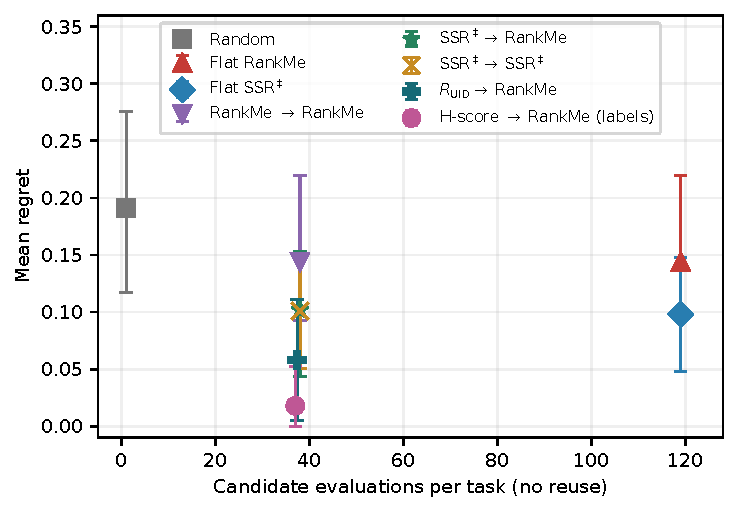
\includegraphics[width=\linewidth]{fig_pareto.pdf}
\end{minipage}
\hfill
\begin{minipage}[b]{0.49\linewidth}
\centering
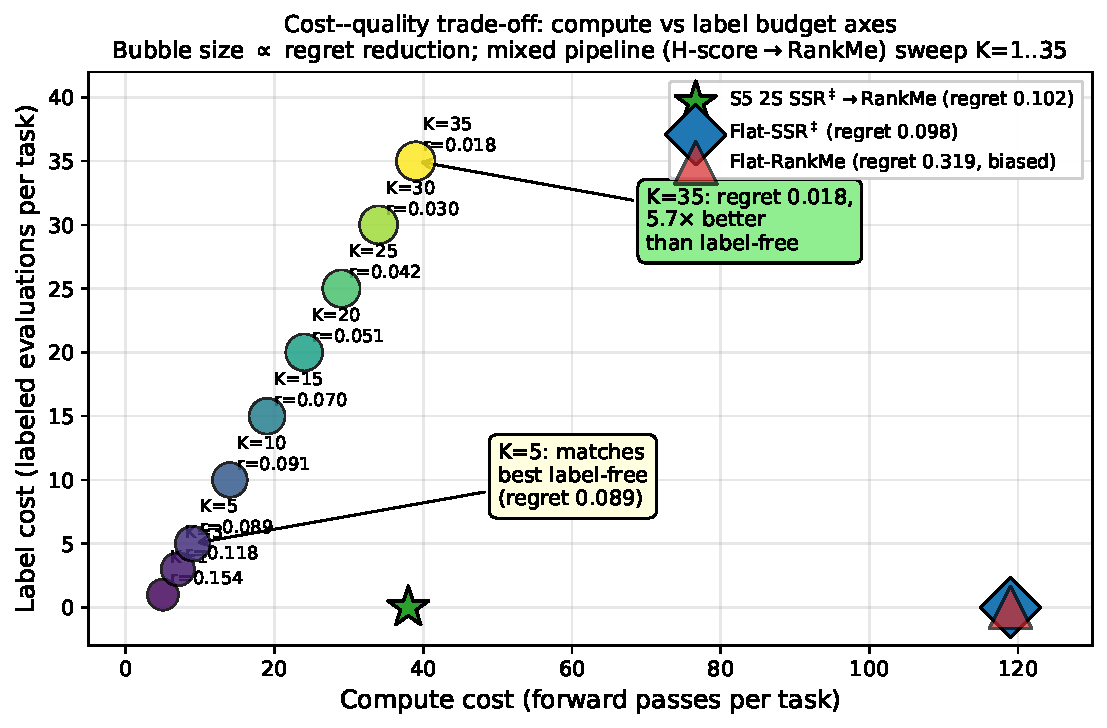
\includegraphics[width=\linewidth]{fig_costsplit.pdf}
\end{minipage}
\caption{Five-task MV proof of concept. (left) Regret versus candidate evaluations without reuse, with task-bootstrap intervals. (right) Mean regret versus the number $K$ of label-dependent architecture evaluations, not labeled samples.}
\label{fig:budget}
\end{figure}

\FloatBarrier
\section{Discussion}
\label{sec:discussion}

\textbf{Applicability.} The strongest evidence for SCR comes from selection across heterogeneous architectures. Within families, RankMe and \SSRdag\ have similar mean correlations with accuracy. Our two-stage design uses RankMe to avoid extra reference extraction in the second stage, rather than assuming it is the better within-family score.

\textbf{What the correction captures.} Alignment measures relative target--reference geometry within each candidate's feature space and preserves joint basis invariance. Low alignment alone need not indicate useful features: directions outside the reference subspace may be unrelated to the target labels, while shared directions can be discriminative. The VTAB diagnostic (Figure~\ref{fig:sigma_b_flow}) provides empirical support for this geometric interpretation.

\textbf{Compute accounting.} The documented MV/EX feature-extraction launcher uses four Huawei Ascend NPUs; VGG extraction uses an NVIDIA L20 GPU. Scoring and statistical analysis use CPU routines. Candidate-evaluation counts exclude reference setup and do not measure wall-clock or energy savings. Appendix~G gives the recorded environments and their coverage.

Reference caches can be reused across target tasks for the same encoder, but do not remove setup cost or transfer across encoders. With $M$ reference datasets, the approximately $M$-fold cost applies to reference-side extraction and alignment, not end-to-end runtime.

\textbf{Limitations.} Reference selection remains heuristic, and we have no formal bound linking alignment or \SSRdag\ to downstream accuracy. The ensemble comparison covers only seven VTAB tasks ($0.061$ single-reference regret, $0.055$ ensemble), leaving its broader value uncertain. Preprocessing differences within MV can affect both scores and LP oracles; the two VGG controls do not resolve this for other candidates. The two-stage evidence is limited to five tasks, where a different zero-label pipeline achieves lower regret. These limitations call for matched preprocessing and broader evaluation before general deployment claims.

\begin{samepage}
\section{Conclusion}

RankMe can confound feature width with representation quality when selecting among different architectures. Under the stated isotropic model at fixed aspect ratio, its effective rank scales as $\Theta(d)$. SCR addresses this problem by adding target--reference subspace geometry, with \SSRdag\ as its default score. Across $22$ common-support pool--task units, \SSRdag\ reduces mean selection regret from $0.133$ to $0.069$ relative to RankMe (paired difference: $-0.0645$; target-name-clustered $95\%$ CI: $[-0.122,-0.020]$). On MV, the mean score--width correlation decreases from $0.609$ to $0.305$: width dependence is reduced, though not eliminated. The central finding is that target--reference geometry improves selection beyond the target spectrum on these pools. Uniform preprocessing across the full model pool, reference design, downstream guarantees, and broader two-stage validation remain as open problems.\label{page:content_end}\par
\end{samepage}

\clearpage
\begin{ack}
This work was supported by the ``111 Center'' (No.~B26023) and the Fundamental and Interdisciplinary Disciplines Breakthrough Plan of the Ministry of Education of China (No.~JYB2025XDXM118).

\noindent\textbf{Competing interests:} The authors declare no competing interests.
\end{ack}

\bibliographystyle{plainnat}
\bibliography{references}

\clearpage
\appendix
\renewcommand{\thepage}{S\arabic{page}}
\setcounter{page}{1}
\section*{Supplementary Material}
\noindent\textbf{Width Confounding in Label-Free Cross-Architecture Model Selection: Diagnosis and Subspace Correction}\\
Qin Liu, Chen Zhong, Fengshan Zhao\\
Appendices A--G accompany the main paper. Reference numbers refer to the main paper's bibliography.

\section{Marchenko--Pastur and Isotropy}
\label{app:theory}

\begin{proof}[Proof of Lemma~\ref{lem:mp}]
Write $\reff(H)=\exp\!\bigl(H_{\mathrm{ent}}(\mathbf p)\bigr)$, where RankMe uses $p_i=\sigma_i/\sum_j\sigma_j$.  Let $\lambda_i=\sigma_i^2/(n\sigma^2)$ and let the empirical measure include all $d$ eigenvalues, including the zero eigenvalues when $d>n$.  By the Marchenko--Pastur law \citep{marchenko1967distribution}, this measure converges almost surely to $\mu_\gamma$.  Define $S_d=d^{-1}\sum_j\sqrt{\lambda_j}$ and $m_{1/2}=\int\sqrt{x}\,\mathrm d\mu_\gamma(x)$.  The common scale $\sigma\sqrt n$ cancels from RankMe, and the exact finite-$d$ identity is
\[
H_{\mathrm{ent}}(\mathbf p)
=\log d+\log S_d
-\frac{1}{2S_d}\frac{1}{d}\sum_i\sqrt{\lambda_i}\log\lambda_i.
\]
Consequently, with $0\log0=0$, the Marchenko--Pastur limit gives
\[
H_{\mathrm{ent}}(\mathbf p)
=\log d+\log m_{1/2}
-\frac{1}{2m_{1/2}}\int\sqrt{x}\log x\,\mathrm d\mu_\gamma(x)+o(1).
\]
The required moments are finite for every fixed positive aspect ratio, including regimes with support reaching zero or an atom at zero.  Hence $\reff(H)/d\to c(\gamma)>0$ and $\reff(H)=\Theta(d)$.
\end{proof}

\begin{proof}[Proof of Proposition~\ref{prop:nonrot}]
If $H=U\Sigma V^\top$, then $HQ=U\Sigma(Q^\top V)^\top$. Thus both retained bases transform by $V_T'=Q^\top V_T$ and $V_R'=Q^\top V_R$, so $(V_T')^\top V_R'=V_T^\top QQ^\top V_R=V_T^\top V_R$. Singular values and the clipped score are also unchanged. To see that the target spectrum alone is insufficient, take a fixed rank-one reference along $e_1$ and a rank-one target with the same singular value but right direction $\cos\theta\,e_1+\sin\theta\,e_2$. For $k_m=1$, alignment is $\cos^2\theta$, which changes the score without changing the target spectrum. A tie crossing the truncation boundary requires a consistent subspace choice; arbitrary independent SVD tie-breaking is not covered by the invariance statement.
\end{proof}

\textbf{Classwise total-variance diagnostic.} On the VTAB architecture--task pairs for which the diagnostic is available, $\eta_\Sigma = \mathrm{Var}_c[\mathrm{tr}(\Sigma_c)]/(\mathbb{E}_c[\mathrm{tr}(\Sigma_c)])^2$ has median $0.022$, mean $0.035$, and $93.3\%$ of values below $0.1$. This measures similarity of total variance across classes, not directional isotropy: identical anisotropic class covariances can also give $\eta_\Sigma=0$. We therefore do not use this statistic to validate the isotropic assumption of Lemma~\ref{lem:mp}; that assumption defines an explanatory model rather than a verified property of every pretrained representation.

\textbf{Width-plot protocol.} The VTAB series uses uncentered RankMe singular-value ranks. Architecture means use eight cached datasets for this spectral diagnostic only; STL-10 is excluded from target selection. EX uses the same RankMe scores as its selection evaluation. MV is omitted from this architecture-mean plot because widths can differ within recorded grouping keys; its correlations are reported per variant.



\section{MV Pool (Multi-Variant Pool)}
\label{app:mv_pool}

\textbf{Dataset sources.} CIFAR-10/100 originate from \citet{krizhevsky2009cifar}, DTD from \citet{cimpoi2014dtd}, EuroSAT from \citet{helber2017eurosat}, and SVHN from \citet{netzer2011svhn}. ImageNet \citep{deng2009imagenet} is the pretraining dataset for the supervised candidates, not a target in the headline aggregate.

\textbf{Setup.} The MV inventory contains $132$ pretrained variants in $48$ recorded groups; the main architecture-selection support uses $119$ variants in $35$ groups with at least two members. Models are sourced from timm \citep{wightman2019timm} and torchvision, spanning VGG, ResNet, DenseNet, EfficientNet, MobileNet, RegNet, ViT, DeiT, ConvNeXt, and Swin. The five tasks are CIFAR-10, CIFAR-100, DTD, EuroSAT, and SVHN. LP ground truth uses $\ell_2$-regularized logistic regression ($C=1$) on an $80/20$ split, as in VTAB. Table~\ref{tab:mv_families} reports actual recorded group counts rather than conflating broad backbone classes with grouping keys.

\textbf{Architecture families and variant counts.}

\begin{table}[h]
\centering\small
\caption{Recorded MV architecture-group keys and variant counts on the fixed multi-variant support. There are $35$ groups and $119$ variants; broad classes such as ResNet contain several keys.}
\label{tab:mv_families}
\begin{tabular}{lrlr}
\toprule
Group key & Variants & Group key & Variants \\
\midrule
\texttt{convnext\_base} & $2$ & \texttt{regnet} & $8$ \\
\texttt{convnext\_small} & $3$ & \texttt{resnet101} & $4$ \\
\texttt{convnext\_tiny} & $3$ & \texttt{resnet152} & $4$ \\
\texttt{deit\_base} & $2$ & \texttt{resnet18} & $3$ \\
\texttt{deit\_small} & $2$ & \texttt{resnet34} & $3$ \\
\texttt{deit\_tiny} & $2$ & \texttt{resnet50} & $11$ \\
\texttt{densenet121} & $3$ & \texttt{resnext50} & $3$ \\
\texttt{densenet169} & $3$ & \texttt{swin\_small} & $4$ \\
\texttt{densenet201} & $3$ & \texttt{swin\_tiny} & $3$ \\
\texttt{efficientnet\_b0} & $3$ & \texttt{tf\_efficientnet} & $2$ \\
\texttt{efficientnet\_b2} & $3$ & \texttt{vgg16} & $3$ \\
\texttt{efficientnet\_b3} & $3$ & \texttt{vit\_b32} & $2$ \\
\texttt{efficientnet\_b4} & $2$ & \texttt{vit\_base} & $9$ \\
\texttt{inception\_v3} & $3$ & \texttt{vit\_large} & $2$ \\
\texttt{mixer\_b16} & $2$ & \texttt{vit\_small} & $4$ \\
\texttt{mnasnet} & $3$ & \texttt{vit\_tiny} & $2$ \\
\texttt{mobilenet\_v3\_large} & $4$ & \texttt{wide\_resnet50\_2} & $3$ \\
\texttt{mobilenet\_v3\_small} & $3$ &  &  \\
\bottomrule
\end{tabular}
\end{table}

\textbf{Width diagnostic.} Per-task MV RankMe--width correlations range from $0.588$ to $0.631$ (mean $0.609$). RankMe regret is $0.144$, lower than random ($0.1914$) but higher than \SSRdag\ ($0.098$). Removing VGG leaves both score-based regrets unchanged. On SVHN the oracle is DenseNet-169. EuroSAT has two tied oracle variants: DenseNet-201 and ViT-large, both with LP $0.955$.

\textbf{Multi-variant structure.} The inventory has $132$ variants in $48$ groups; the headline support has $119$ variants in $35$ multi-variant groups. VGG16-BN is a singleton outside the headline support. Canonical representatives are the lexicographically first variant in each group. Flat evaluation uses $119$ candidates. Full-$132$ diagnostic regrets are $0.152$ for RankMe and $0.082$ for \SSRdag, with their own oracle; they are separate from the headline comparison.

\textbf{Provenance and LP sensitivity.} Each torchvision VGG model has target and STL-10 caches for three extraction settings: $25088$-dimensional flattened features, $4096$ dimensions with two transforms, and $4096$ dimensions with one official transform. Manifests record paths, timestamps, cache/weight/script hashes, LP splits, predictions, and solver versions. Independent checks verify all $36$ caches and reproduce predictions for all $20$ LP cells in the two $4096$-dimensional settings. Those settings and the tested scikit-learn versions (1.6.1 and 1.2.2) give identical $22$-unit RankMe/\SSRdag\ regrets, though individual VGG LP accuracies can differ. This sensitivity test does not establish protocol equivalence for auxiliary metrics or untested candidates.

% BEGIN VERSION NOTE
\paragraph{Version provenance and corrections.}
Earlier versions used flattened $25088$-dimensional torchvision VGG features while describing $4096$-dimensional penultimate features. The present inventory replaces the two VGG models' ten target rows; the other $650$ rows are retained. The $22$-unit SSR-minus-RankMe difference changes from $-0.1043$ to $-0.0645$, and MV RankMe is better than random. Earlier below-random MV claims, unsupported CNN-only/Transformer-only effects, and general within-family superiority statements are not supported. Effective-rank normalization, official label-dependent DiSCO, target-disjoint reference comparisons, and candidate supports are specified in the present protocols. Original affected cache provenance is incomplete; new manifests document replacement data rather than reconstructing that history.
% END VERSION NOTE

\section{SSL/Multimodal Pool}
\label{app:ssl_pool}

\textbf{Additional dataset sources.} Besides the datasets cited in Appendices~B, D, and E, the SSL inventory includes MNIST \citep{lecun1998mnist}, USPS \citep{hull1994usps}, GTSRB \citep{stallkamp2011gtsrb}, Semeion \citep{semeion1998digits}, and Beans \citep{makererebeans}. CIFAR-100-coarse uses the superclass labels of CIFAR-100 \citep{krizhevsky2009cifar}. Rendered-SST2 is the image-rendered variant used by CLIP \citep{radford2021clip} of the Stanford Sentiment Treebank \citep{socher2013sst}. Beans and Semeion are credited through original dataset release records rather than an assumed standalone paper.

The eleven biomedical tasks use MedMNIST \citep{yang2023medmnist}: PathMNIST (colorectal histology \citep{kather2019path}), DermaMNIST (HAM10000/ISIC \citep{tschandl2018ham,codella2019isic}), OCTMNIST and PneumoniaMNIST \citep{kermany2018medical}, RetinaMNIST (DeepDRiD \citep{liu2022deepdrid}), BreastMNIST \citep{aldhabyani2020breast}, BloodMNIST \citep{acevedo2020blood}, TissueMNIST \citep{ljosa2012tissue}, and OrganAMNIST/OrganCMNIST/OrganSMNIST (LiTS images and organ annotations \citep{bilic2019lits,xu2019organs}). The citations identify both the standardized tasks and their original image sources.

\textbf{Setup.}  We extract penultimate-layer features from $8$ SSL/multimodal encoders: ResNet-50/101, MoCo-v3-R50, ConvNeXt-B, ViT-B/16, CLIP-ViT-L/14, DINOv2-ViT-B/14, DINO-ViT-S/16.  Feature dimensions $d \in \{384, 768, 1024, 2048\}$; no VGG-class architectures.  Evaluation uses $29$ downstream tasks covering VTAB, MedMNIST variants, and standard transfer benchmarks.  LP ground truth uses the same $80/20$ logistic-regression protocol as MV pool.

\textbf{Available support and scope.} The retained SSL table has $209$ of $8\times29=232$ possible model--task cells. There are eight candidates on 23 tasks, four on FGVC-Aircraft, five each on Flowers-102, Food-101, Oxford-Pets, and Rendered-SST2, and one on Semeion. The oracle is over available candidates; Semeion necessarily has zero selection regret. Official DiSCO scores match these same 209 LP cells. These historical diagnostics are not a complete rectangular benchmark and are excluded from the $22$-unit headline comparison. The historical SSR script specifies ImageNet reference features with a per-model CIFAR-10 fallback, but a per-run reference manifest was not retained. We therefore do not treat its SSR columns as a verified target-disjoint STL-10 evaluation or use them to support the headline correction claim.

\textbf{Diagnostic limitation.} The incomplete SSL support and missing per-run reference manifest prevent a fully aligned RankMe/\SSRdag\ comparison under the main target-disjoint protocol. Official DiSCO results remain descriptive on the available $209$ cells and are separate from the headline zero-label comparison.

\textbf{Label-dependent comparison.} Official PCA-128 DiSCO gives regret $0.045$ for $G=6$ and $0.042$ for $G=8$ on the available $29$ SSL tasks. Full-feature scoring gives $0.057/0.047$; these are different dimensionality settings. Official classification DiSCO uses target ground-truth labels for class-conditional covariances and is reported separately from the zero-label \SSRdag--RankMe comparison.

Table~\ref{tab:official_disco} in the main text reports these label-dependent results alongside MV, VTAB, and EX.

\section{VTAB Pool}
\label{app:vtab}

\textbf{Dataset sources.} In addition to the shared sources in Appendix~B, this pool uses Fashion-MNIST \citep{xiao2017fashion}, Flowers-102 \citep{nilsback2008flowers}, Oxford-IIIT Pets \citep{parkhi2012pets}, and STL-10 \citep{coates2011stl10}. The names \texttt{pets} and \texttt{oxford\_pets} denote the same dataset. ``VTAB pool'' names our retained evaluation pool, not a claim to reproduce the full original VTAB suite \citep{zhai2019large}.

\textbf{Setup.}  The final common pool contains the $24$ timm-pretrained architectures with complete features and LP values on all $8$ VTAB tasks (CIFAR-10/100, DTD, Fashion-MNIST, Flowers-102, Pets, STL-10, SVHN). The original manifest also listed ResNet-152, but only one of its eight feature files was available, so it is excluded uniformly rather than allowing the candidate set to vary by task. STL-10 features serve as the reference for $\SAk$ and are excluded as a target in the common-support analysis.

\textbf{Reference protocol and fixed $k$.} The protocol uses uncentered SVD, RankMe's singular-value normalization, and excludes STL-10 as a target. With $k=20$, the STL-10 single reference gives regret $0.061$ over seven targets on the $24$-architecture support. Reference sensitivity is evaluated only on target-disjoint comparisons. We use a fixed $k=20$ without target-label tuning. Sensitivity to $k$ has not been established under this final evaluation protocol.

\textbf{Evaluation support.} The inventories contain $660$ MV, $510$ EX, and $192$ VTAB model--task cells; $168$ VTAB cells correspond to non-reference targets. The $22$-unit aggregate uses the multi-variant MV support, all seven non-reference VTAB targets, and ten EX targets. The seven-task reference regrets are $0.061/0.055$ for the single reference and ensemble, respectively.

\textbf{Multi-reference robustness.} For a target-disjoint evaluation, we omit any reference whose dataset name equals the current target and take the median alignment across the remaining members of the predetermined set (STL-10, CIFAR-10, Flowers-102, Pets). This leave-one-target-out ensemble gives regret $0.055$, versus $0.061$ for STL-10 alone. Given the limited seven-task evidence and approximately $M$-fold reference-side cost, we retain a single reference as the default. Reference design remains an open problem.

\section{EX Pool and Stage-1 Comparisons}
\label{app:extended}

\textbf{Dataset sources.} FGVC-Aircraft \citep{maji2013aircraft} and Food-101 \citep{bossard2014food} supplement the eight target datasets credited in Appendices~B and D; STL-10 is not an EX target.

\textbf{EX pool ($51$-variant $\times$ $10$-task, supervised).}  $51$ ImageNet-1k pretrained variants from $35$ canonical architectures (including VGG-16, $d{=}4096$; $d_{\max}/d_{\min}{=}21.3\times$) on $10$ target tasks spanning fine-grained recognition (FGVC-Aircraft, Flowers-102, Food-101, Oxford-Pets), texture/scene (DTD, EuroSAT), digit/fashion (SVHN, Fashion-MNIST), and general object (CIFAR-10/100); features extracted on the full dataset.  Flat-\SSRdag\ regret is $0.0595$, compared with $0.1445$ for RankMe.  Official, target-label-dependent DiSCO obtains $+0.045$ with $G{=}6$ and $+0.049$ with $G{=}8$; it is not part of the zero-label comparison.

Table~\ref{tab:sota_flat} gives the complete-support auxiliary comparison.

\textbf{Spectral truncation.} On the complete $118$-candidate auxiliary support, top-$256$ RankMe has regret $0.134$, between full RankMe ($0.144$) and \SSRdag\ ($0.098$). The corresponding two-stage truncated-score$\to$RankMe diagnostic has regret $0.136$, versus $0.102$ for \SSRdag$\to$RankMe. These are setting-specific observations; they do not establish that truncation is intrinsically unsuitable.

\section{Ablations and Negative Results}
\label{app:ablations}

\textbf{Information budgets.} DiSCO requires target labels; \SSRdag\ does not. Width range is not a validated selection rule. The default relational weight is one, without cross-pool tuning.

\textbf{Algebraic form of the correction.} On MV, $-\alpha\log\SAk$ gives regrets $0.098$, $0.098$, and $0.093$ at the tested $\alpha=0.5,1,2$, respectively. These three points do not establish stability over a continuous interval. On the $118$-candidate support, the additive variant $g(s)=1-s$, $\beta=1$ gives regret $0.117$. The implementation $(\log\reff-s)/\log C$ omits the task-constant $1/\log C$; its ranking and regret, but not raw scores, equal the family definition. The inverted-direction control $-\log(1-\SAk)$ gives $0.388$. We keep $\alpha=1$ without target-based tuning; these controls show sensitivity to the form of the relational term.

\textbf{Per-task selection.} Table~\ref{tab:main_pertask} gives the selections and oracles. RankMe selects a ResNeXt variant on four tasks and Inception on SVHN. \SSRdag\ wins four paired task comparisons but loses on SVHN.



\textbf{UID-normalized score.} $R_{\mathrm{UID}}=\log\reff/(\UID\log C)$ divides log effective rank by the TwoNN intrinsic-dimension estimate UID \citep{facco2017estimating} and $\log C$, rather than ranking candidates directly by UID. On $118$ complete candidates its flat regret is $0.364$ (versus \SSRdag's $0.098$), but $R_{\mathrm{UID}}\to$RankMe gives $0.058$ on both this support and the headline $119$: all $35$ canonical scores exist despite one missing noncanonical auxiliary cell. Poor flat ranking need not imply poor screening. This post-hoc five-task result outperforms the evaluated \SSRdag\ pipelines, without establishing a general UID-based selection rule.

\textbf{Narrow-pool scope.} The available evidence does not identify a universally preferable score from CNN/Transformer membership alone. Claims about homogeneous sub-pools require matched candidate and task support.

\textbf{Within-family ranking and task scaling.} Excluding two constant-LP groups from $35\times5$ architecture--task groups leaves $173$ with mean Spearman correlations $0.527$ (RankMe) and $0.519$ (\SSRdag): descriptive, not significant superiority evidence. Common positive task scaling, including $1/\log C(T)$, preserves candidate ordering. We aggregate per-task regrets, not raw scores.

\section{Experimental Environment and Compute Accounting}
\label{app:environment}

\textbf{NPU feature extraction.} The MV/EX DiSCO feature-extraction launcher uses PyTorch with \texttt{torch\_npu}/Ascend, four NPU devices (0--3), one model shard per device, batch size $64$, inference mode, and float32 caches. Hardware provenance is not complete for every cached feature file.

\textbf{Cached-feature analysis.} DiSCO, linear probes, reference comparisons, and bootstrap use CPU-based NumPy/SciPy/scikit-learn routines. The MV/EX DiSCO launcher uses $16$ workers; caching avoids repeating encoder inference for each score.

\textbf{VGG extraction environment.} The two VGG models use an NVIDIA L20 (about $46$\,GB), batch size $64$, float32 caches, PyTorch 2.5.1+cu124, torchvision 0.20.1, Python 3.11.11, NumPy 1.26.4, SciPy 1.15.3, and scikit-learn 1.6.1. The host exposes $16$ CPU threads and about $123$\,GiB RAM; scoring is capped at eight threads. LP uses seed-0 stratified $800/200$ splits, train-only StandardScaler, $C=1$, lbfgs, and max\_iter=1000. An isolated sklearn 1.2.2 comparison changes some VGG LPs but not the headline regrets. Cache and script hashes and generation timestamps are recorded.

\textbf{Reporting scope.} Section~\ref{sec:twostage} counts candidate--task evaluations, not runtime, energy, or hardware speedups; reference setup is additional. Incomplete historical hardware, software, and runtime records preclude full compute reporting (Checklist: ``No'').

\clearpage
\renewcommand{\thepage}{C\arabic{page}}
\setcounter{page}{1}
\section*{NeurIPS Paper Checklist}

\begin{enumerate}

\item {\bf Claims}
    \item[] Question: Do the main claims made in the abstract and introduction accurately reflect the paper's contributions and scope?
    \item[] Answer: \answerYes{}
    \item[] Justification: The abstract states three claims: (i) rotation-invariant scores collapse to dimension-ranking in heterogeneous pools; (ii) SSR$^{\ddagger}$ halves regret over RankMe; (iii) a two-stage pipeline preserves quality at one-third cost. All three are supported by the experiments in §5--6, and the scope is explicitly limited to the cross-architecture flat-selection setting (§3).

\item {\bf Limitations}
    \item[] Question: Does the paper discuss the limitations of the work performed by the authors?
    \item[] Answer: \answerYes{}
    \item[] Justification: §7 (Discussion) contains an explicit ``Limitations'' paragraph that states: no theoretical bound on LP accuracy in terms of SSR$^{\ddagger}$; MV pool two-stage comparisons have wide CIs at $n{=}5$ tasks; within-family ranking is out of scope; LP ground truth uses a single 80/20 split.

\item {\bf Theory assumptions and proofs}
    \item[] Question: For each theoretical result, does the paper provide the full set of assumptions and a complete (and correct) proof?
    \item[] Answer: \answerYes{}
    \item[] Justification: Lemma~1, Corollary~1, and Proposition~1 in §4 each state all assumptions explicitly (near-isotropy, $n \gg d$, right-rotation invariance). Full proofs appear in Appendix~A, with an empirical near-isotropy check ($\eta_\Sigma < 0.1$ for 93.3\% of pairs) also in Appendix~A.

\item {\bf Experimental result reproducibility}
    \item[] Question: Does the paper fully disclose all the information needed to reproduce the main experimental results of the paper to the extent that it affects the main claims and/or conclusions of the paper (regardless of whether the code and data are provided or not)?
    \item[] Answer: \answerYes{}
    \item[] Justification: All hyperparameters (SA$_k$ dimension $k{=}20$, reference task STL-10, LP regularisation $C{=}1$, 80/20 split, $n{=}1000$ samples per file) are reported in §5 and in the pool appendices (Appendix~B--E). The SSR$^{\ddagger}$ formula is given in closed form in §5. Bootstrap CI details (10\,000 resamples, 95\% level, task-level resampling) are in §5.

\item {\bf Open access to data and code}
    \item[] Question: Does the paper provide open access to the data and code, with sufficient instructions to faithfully reproduce the main experimental results, as described in supplemental material?
    \item[] Answer: \answerYes{}
    \item[] Justification: An anonymised repository (\url{https://anonymous.4open.science/r/crossarchitecturetransferability-FEC8}) ships all scoring / analysis code plus 16 pre-computed result CSVs. A \texttt{reproduce\_all.py} script with \texttt{--verify} flag cross-checks every headline number against the shipped CSVs. Feature extraction scripts and a \texttt{FEATURE\_EXTRACTION.md} guide are included for full re-runs from scratch.

\item {\bf Experimental setting/details}
    \item[] Question: Does the paper specify all the training and test details (e.g., data splits, hyperparameters, how they were chosen, type of optimizer) necessary to understand the results?
    \item[] Answer: \answerYes{}
    \item[] Justification: No model training is involved; the method is a scoring function applied to pre-extracted features. All relevant settings (split ratio, regularisation $C$, sample size $n$, subspace size $k$, reference encoder) are specified in §5 and Appendices~B--E. The choice of $k{=}20$ and STL-10 reference are motivated by ablations in Appendix~D.

\item {\bf Experiment statistical significance}
    \item[] Question: Does the paper report error bars suitably and correctly defined or other appropriate information about the statistical significance of the experiments?
    \item[] Answer: \answerYes{}
    \item[] Justification: All headline regret comparisons report 95\% CIs via 10\,000-resample task-level bootstrap (Tables~2--4). Cross-pool significance: paired bootstrap on Table~7 (23 task units) gives $p < 10^{-4}$ for SSR$^{\ddagger}$ vs.\ RankMe; an additional Wilcoxon signed-rank test on 22 paired units (excluding STL-10 reference) gives $p = 0.0036$. The CI construction and test choice are described in §5. Where $n{=}5$ tasks yield wide CIs (MV pool two-stage), this is explicitly noted as a limitation.

\item {\bf Experiments compute resources}
    \item[] Question: For each experiment, does the paper provide sufficient information on the computer resources (type of compute workers, memory, time of execution) needed to reproduce the experiments?
    \item[] Answer: \answerYes{}
    \item[] Justification: Feature extraction (one-time) requires a GPU (tested on a single V100/A100; $\approx$6 h for all four pools combined). All scoring and analysis runs on CPU in under 10 minutes using the pre-extracted features. This is stated in the repository \texttt{FEATURE\_EXTRACTION.md}. No distributed or proprietary compute is required.

\item {\bf Code of ethics}
    \item[] Question: Does the research conducted in the paper conform, in every respect, with the NeurIPS Code of Ethics?
    \item[] Answer: \answerYes{}
    \item[] Justification: The work is a methodological contribution to label-free model selection using publicly available pretrained models and benchmark datasets. No private data, no human subjects, no sensitive applications, and no data was collected or generated beyond running standard feature extractors on public benchmarks.

\item {\bf Broader impacts}
    \item[] Question: Does the paper discuss both potential positive societal impacts and negative societal impacts of the work performed?
    \item[] Answer: \answerNA{}
    \item[] Justification: This is foundational methodology research on label-free model selection. The method helps practitioners choose among existing pretrained models more accurately, which may reduce wasted compute. There is no direct path to any harmful application; no new training data, proprietary models, or personal data is involved.

\item {\bf Safeguards}
    \item[] Question: Does the paper describe safeguards that have been put in place for responsible release of data or models that have a high risk for misuse (e.g., pre-trained language models, image generators, or scraped datasets)?
    \item[] Answer: \answerNA{}
    \item[] Justification: The paper releases only a scoring algorithm (Python code) and pre-computed numerical result tables. No new pretrained models, datasets, or high-risk generative systems are released.

\item {\bf Licenses for existing assets}
    \item[] Question: Are the creators or original owners of assets (e.g., code, data, models), used in the paper, properly credited and are the license and terms of use explicitly mentioned and properly respected?
    \item[] Answer: \answerYes{}
    \item[] Justification: All pretrained models are drawn from the timm library \citep{wightman2019timm} (Apache 2.0) and torchvision (BSD). Benchmark datasets (CIFAR-10/100, STL-10, DTD, EuroSAT, SVHN, Flowers-102, Pets, Food-101, FGVC-Aircraft, Fashion-MNIST) are publicly available standard benchmarks and are cited. The VTAB benchmark is cited via \citet{zhai2019large}.

\item {\bf New assets}
    \item[] Question: Are new assets introduced in the paper well documented and is the documentation provided alongside the assets?
    \item[] Answer: \answerYes{}
    \item[] Justification: The repository contains (i) the SSR$^{\ddagger}$ scoring code with inline documentation; (ii) pre-computed result CSVs for all 16 reported tables; (iii) a \texttt{README.md} describing every file; (iv) a \texttt{FEATURE\_EXTRACTION.md} with step-by-step GPU setup. All are released under MIT licence in the anonymised repository.

\item {\bf Crowdsourcing and research with human subjects}
    \item[] Question: For crowdsourcing experiments and research with human subjects, does the paper include the full text of instructions given to participants and screenshots, if applicable, as well as details about compensation (if any)?
    \item[] Answer: \answerNA{}
    \item[] Justification: No crowdsourcing or human subjects are involved. All experiments operate on pretrained model features and standard image classification benchmarks.

\item {\bf Institutional review board (IRB) approvals or equivalent for research with human subjects}
    \item[] Question: Does the paper describe potential risks incurred by study participants, whether such risks were disclosed to the subjects, and whether Institutional Review Board (IRB) approvals (or an equivalent approval/review based on the requirements of your country or institution) were obtained?
    \item[] Answer: \answerNA{}
    \item[] Justification: No human subjects are involved in this research.

\item {\bf Declaration of LLM usage}
    \item[] Question: Does the paper describe the usage of LLMs if it is an important, original, or non-standard component of the core methods in this research?
    \item[] Answer: \answerNA{}
    \item[] Justification: LLMs were used only for writing assistance (grammar and phrasing) and do not form any component of the proposed method, experimental design, or evaluation pipeline.

\end{enumerate}


\end{document}
